\documentclass[a4paper,11pt]{article}
\usepackage{amsmath,amssymb}
\usepackage[a4paper,left=19mm,right=19mm,top=40mm,bottom=40mm]{geometry}
\usepackage{txfonts}
\usepackage{kotex}
\usepackage{graphicx}
\usepackage{algorithm}
\usepackage{algpseudocode}
\usepackage{fancyvrb}

\begin{document}
\title{자료구조 HW9}
\author{B935394 컴퓨터공학과 장준희}
\maketitle
\newpage
\section{Maxheap의 삽입과 삭제}
\ \ Maxheap의 삽입과 삭제에 대해 알아보기 위해서는 우선 Maxheap이 무엇인지 알아야한다.\\
\begin{figure}[h]
\begin{center}

\includegraphics[width=\textwidth]{maxheap}
\caption{Maxheap}
\label{fig:fig1}
\end{center}
\end{figure}
\\Maxheap은 위의 그림처럼 \textbf{최대트리}와 \textbf{완전이진트리}를 만족해야한다.이에 유의하면서 삽입과 삭제를 알아보면,
우선 삽입은 가장 마지막 노드에 일단 삽입한 후, 부모노드와 비교를 통해 최대트리가 될 때까지 올려보내는 과정이다. 그림으로 보면 다음과 같다.
\begin{figure}[h]
\begin{center}
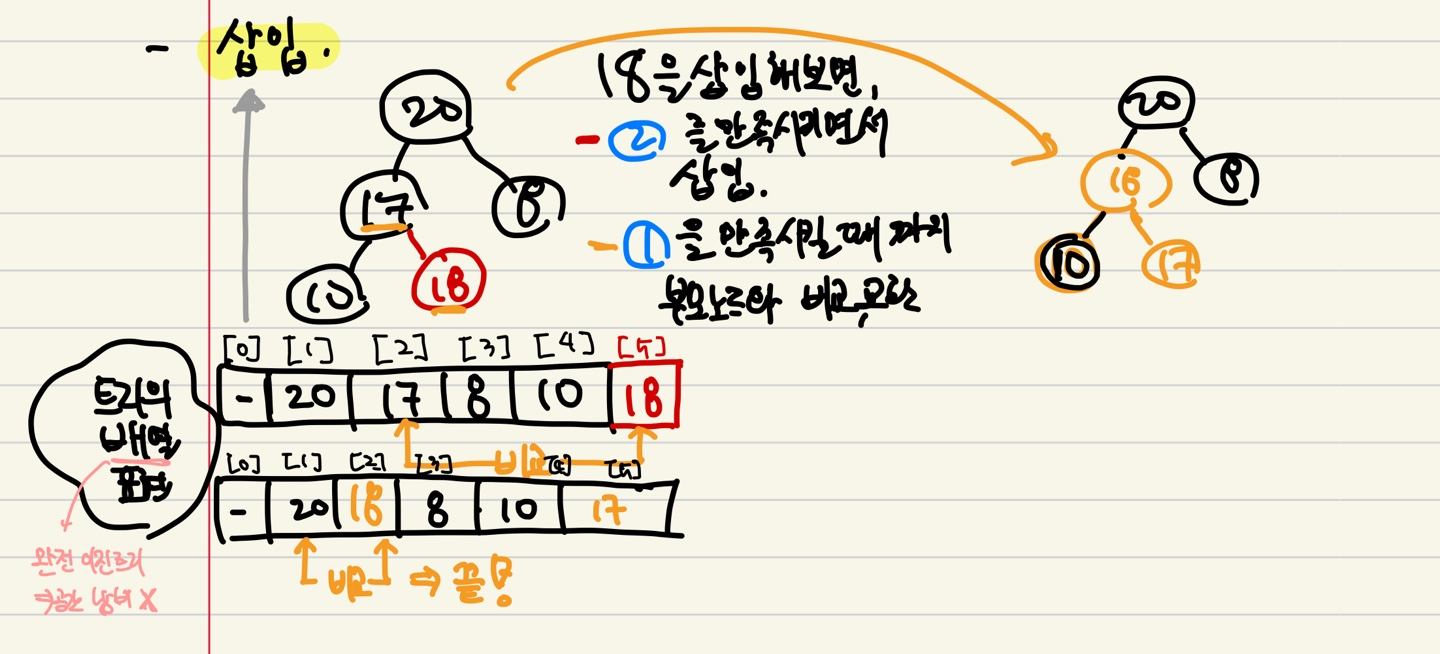
\includegraphics[width=\textwidth]{insert}
\caption{Insert}
\label{fig:fig2}
\end{center}
\end{figure}
\\그림에서 볼 수 있듯이 일단 18을 맨 마지막 노드에 삽입한 후, 17(부모노드)와의 비교를 통해 올려보내고 또 20과 비교를 한 후 올리지 않고 끝내는 것을 볼 수 있다.
\newpage 삭제의 경우는 우선 루트노드를 제거하고, 가장 마지막 노드를 루트노드의 위치로 올린다음, 자식노드와의 비교를 통해 최대트리가 될 때까지 내려보내는 과정이다. 그림으로 보면 다음과 같다.

\begin{figure}[h]
\begin{center}
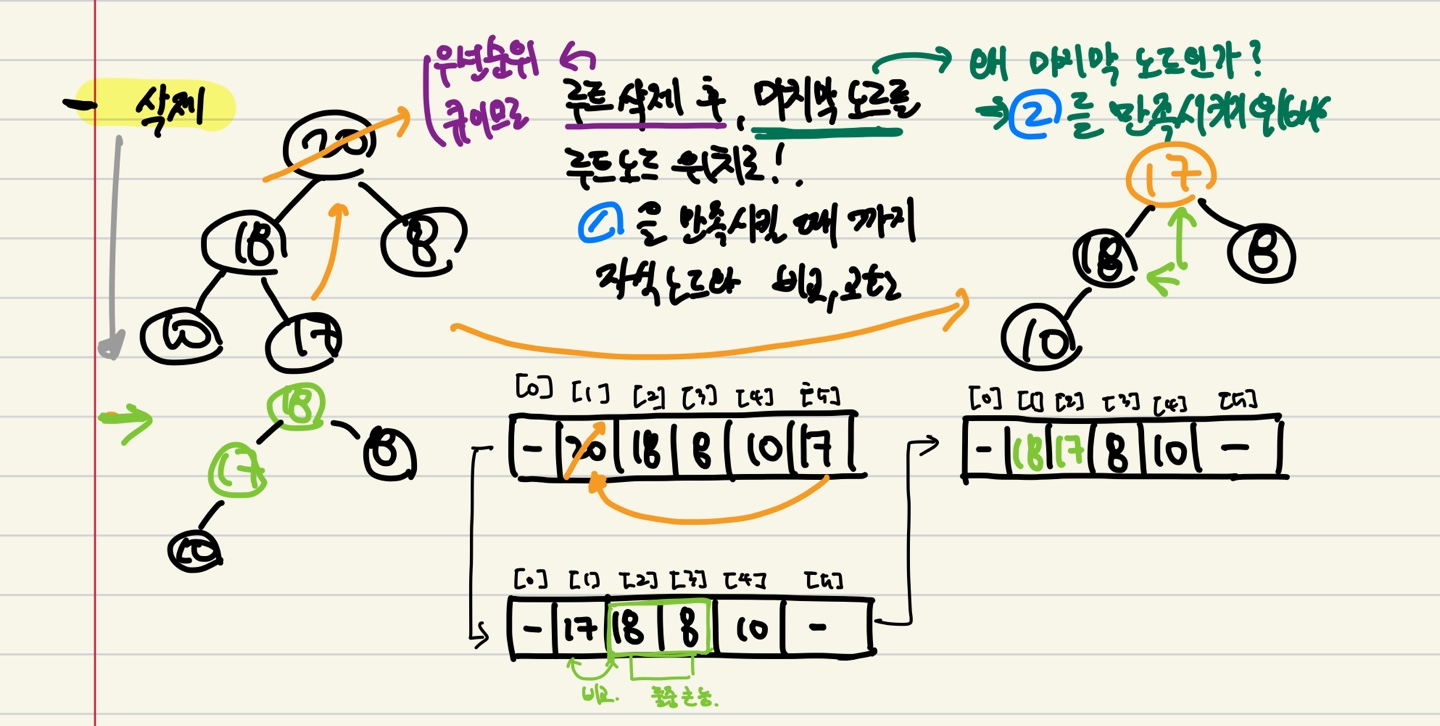
\includegraphics[width=\textwidth]{delete}
\caption{Delete}
\label{fig:fig3}
\end{center}
\end{figure}

그림에서처럼 20(루트노드)를 일단 제거하고 17(가장 마지막 노드)를 루트노드로 올린다. 그 후 18(자식노드)와의 비교를 통해 17을 내려보내고 18을 올려보낸다. 그 후 다시 10과의 비교(17의 자식노드)를 한 후 최대트리를 만족하므로 멈춘다.

\section{코드 설명}

\ \ 우선 이번 Maxheap의 구현 같은 경우 이전 과제들과는 달리 트리를 표현하는데 배열을 사용하였다. 즉, 배열이 트리이고 배열의 원소가 각 노드이다. 트리의 표현이 어떻게 되었는지는 \ref{fig:fig1}을 보면, 배열과 트리 둘 다 표현되어있으므로 비교하면 알 수 있다. 이제 코드를 보면, 다음과 같다.
\begin{Verbatim}
------------------------------------------------------------------------------
template <class T>
class Maxheap		//Maxheap은 기본적으로 큐이다.
{
private:
    void ChangeSize1D(int);	//트리 크기 변경
    T *heap;		//동적할당 된 트리배열을 가리키는 포인터
    int heapSize;		//현재 힙의 크기
    int capacity;		//저장 가능한 노드의 수:배열칸수-1(왜냐하면 [0]은 공란)

public:
    Maxheap(int);		//생성자
    void Push(const T &);		//insert기능
    void Pop();	//delete 기능
    bool IsEmpty() { return heapSize == 0; }	//힙이 비어있는가?
    T Top() { return heap[1]; }	//루트노드 반환
    template <class T2>
    friend ostream &operator<<(ostream &, Maxheap<T2> &);
};
------------------------------------------------------------------------------
template <class T>
void Maxheap<T>::ChangeSize1D(int size)
{ //heap의 크기를 size만큼 늘리는 함수.
    if(size<=0)throw"추가하고자하는 크기는 양수여야합니다";
    T*temp = new T[size+capacity+1];      //늘리고자하는 size, 노드저장가능개수, [0]
    int number=size;
    copy(heap,heap+capacity+1,temp);		
    //algorithm의 함수 기존힙(heap이 가리키는)을 확장된 힙(temp가 가리키는)에 복사.
    delete [] heap;		//heap이 가리키고 있는 기존 힙 반환
    heap=temp;		//temp가 가리키는 배열을 heap이 가리키게 함
}
------------------------------------------------------------------------------
template <class T>
void Maxheap<T>::Push(const T &newdata)
{
    if(heapSize==capacity){ 	//만약 더 노드를 삽입할 수 없으면 확장
        ChangeSize1D(capacity+1);
        capacity*=2;
    }
    int currentNode=++heapSize; //현재 힙의 가장 첫 공란위치.
    while(currentNode!=1&&heap[currentNode/2]<newdata){ 
    		//현재 노드의 데이터가 삽입될 데이터보다 작고 루트 노드가 아니라면 
        heap[currentNode]=heap[currentNode/2];  //부모를 내려보낸다
        currentNode /=2;
    }
    heap[currentNode]=newdata;		//공란에 새 데이터 추가.
}
------------------------------------------------------------------------------
template <class T>
void Maxheap<T>::Pop()
{//delete max element
    if(IsEmpty()) throw "heap is empty. Cannot Delete";
    heap[1].~T();//delete max element
    T lastE = heap[heapSize--]; 
    //힙의 마지막 노드의 값을 받아두고, 없앤다.(남아있지만, 접근불가)

    //내려보내는 과정할 준비
    int currentNode=1;  //root
    int child=2;    //a child of currentNode
    while(child<=heapSize){ //아들이 있는 경우     
        //두 자식 노드 중 값이 큰 노드를 비교대상으로 한다.
        if(child<heapSize&&heap[child]<heap[child+1])child++;
        //자식노드보다 크다면 그 위치에 값을 넣는다.
        if(lastE>=heap[child])break;

        heap[currentNode]=heap[child];  //그게 아니라면 자식을 올린다
        currentNode=child;child*=2;     //아래 레벨로 내려간다.
    }
    heap[currentNode]=lastE;	//조건을 만족하면 값을 넣는다.
}
------------------------------------------------------------------------------
template <class T>
ostream &operator<<(ostream &os, Maxheap<T> &H)
{
    os << "<Heap contents> ";
    int i;
    for (i = 1; i <= H.heapSize; i++)
        os << i << ":" << H.heap[i] << " ";
    os << endl;
}		//Maxheap출력 연산자 오버로딩
------------------------------------------------------------------------------
template <class T>
Maxheap<T>::Maxheap(int _capacity = 10) : heapSize(0)
{
    if (_capacity < 1)
        throw " Must be > 0";
    capacity = _capacity;
    heap = new T[capacity + 1];     //[0]을 비워두기 때문!!
}
------------------------------------------------------------------------------
\end{Verbatim}
\section{기타}
\begin{itemize}
\item $<<$연산자 오버로딩에서 반환값이 ostream\&으로 존재하는데, 구현부에서 return이 없는데 내 pc상에서는 안돌아가고 학교 서버 상에서 잘 실행되는 이유를 모르겠다.
\end{itemize}

\end{document}